\section{Разработка программной поддержки для взаимодействия с адресной светодиодной лентой}
\label{sec:develop}

\subsection{Постановка задач на проектирование}
\label{sec:develop:task}

Задачей дипломного проекта является разработка и создание мобильного приложения для управления световым оборудованием (адресной светодиодной лентой). 

Основная цель разработки программного продукта – улучшение пользовательского опыта при управлении гирляндами (адресными светодиодными лентами).
Разрабатываемая система должна удовлетворять следующим требованиям:
\begin{itemize}
	\item хранение данных должно быть обеспечено с помощью мобильной базы данных Realm;
	\item должна быть реализована возможность удаленной работы с адресной лентой через подключение к ней как напрямую по Wi-Fi, так и через стороннюю Wi-Fi точку;
	\item должна быть реализована возможность создания и удаления пользовательских анимаций, а также редактирования стандартных анимаций (изменение скорости анимации, частоты лампочек и набора цветов);
	\item должна быть реализована возможность отправки своих анимаций другим пользователям;
	\item должна быть реализована возможность регистрации пользователей (база пользователей используется для отправки анимаций);
	\item должна быть реализована возможность объединения адресных лент в одну сеть для последующего единого управления;
	\item должна быть реализована возможность обновления прошивки лент с мобильного телефона;
	\item взаимодействие мобильного приложения должно осуществляться посредством протоколов HTTP, TCP/IP и UDP.
\end{itemize}

Для авторизации пользователей, отправки анимаций и обновления прошивки должен быть реализован сторонний сервер, который будет управлять обменом данных между мобильными приложениями.


\newpage
\subsection{Обоснование принимаемых решений по выбору методов и средств реализации}
\label{sec:develop:functionalModel}

Язык программирования, на котором будет реализована система, заслуживает большого внимания, так как вы будете погружены в него с начала конструирования программы до самого конца. Исследования показали, что выбор языка программирования несколькими способами влияет на производительность труда программистов и качество создаваемого ими кода \cite{code_complete}. Если язык хорошо знаком программистам, они работают более производительно. Данные, полученные при помощи модели оценки Cocomo II, показывают, что программисты, использующие язык, с которым они работали три года или более, примерно на 30\% более продуктивны, чем программисты, обладающие аналогичным опытом, но для которых язык является новым~\cite{software_cost_estimation}. В более раннем исследовании, проведенном в IBM, было обнаружено, что программисты, обладающие богатым опытом использования языка программирования, были более чем втрое производительнее программистов, имеющих минимальный опыт~\cite{method_of_programming_measurement_and_estimation}.

Язык программирования Swift является кроссплатформенным языком программирования, разработанный Apple Inc. для iOS, macOS, watchOS, tvOS и Linux. Swift предназначен для работы с фреймворками Apple Cocoa и Cocoa Touch и большим объемом существующего кода на  Objective-C (ObjC), написанного для продуктов Apple. Он построен с использованием компилятора LLVM с открытым исходным кодом и включен в Xcode с версии 6. На платформах, отличных от Linux, он использует библиотеку времени выполнения Objective-C, которая позволяет использовать C, Objective-C, C ++ и Swift в рамках одной программы \cite{objc_doc}.

Apple стремилась в Swift поддержать многие основные концепции, связанные с Objective-C, в частности динамической рассылкой, широко распространенной поздней привязкой, расширяемым программированием и аналогичными функциями, а также сделать язык \enquote{более безопасным} (проще поймать программные ошибки) \cite{mobx_best_practices}. Swift пытается решить проблемы, связанные с некоторыми распространенными ошибками программирования, такими как нулевые указатели, и обеспечивает синтаксический сахар, чтобы избежать этих ошибок. Swift поддерживает концепцию расширяемости протокола, систему расширяемости, которая может применяться к типам, структурам и классам, которые Apple рекламирует как реальное изменение в парадигмах программирования, которые они называют \enquote{протокольно-ориентированным программированием} \cite{swift_doc}.

Во многих объектно-ориентированных языках объекты представлены двумя частями. Объект хранится как блок данных, помещенных в кучу, тогда как имя (или «дескриптор») к этому объекту представляется указателем. Объекты передаются между методами путем копирования значения указателя, позволяя тем самым не копировать сами данные. В тоже время, основные типы, такие как целые числа и значения с плавающей запятой, представлены без ссылок; дескриптор содержит данные, а не указатель на него, и эти данные передаются непосредственно путем копирования \cite{swift_doc}.

Обе концепции имеют свои преимущества и недостатки. Объекты полезны, когда данные большие, например, описание окна или содержимого документа. В этих случаях доступ к этим данным обеспечивается путем копирования 32- или 64-битного значения по сравнению с копированием всей структуры данных. Однако меньшие значения, такие как целые числа, имеют тот же размер, что и указатели (как правило, оба являются одним словом), поэтому нет никакого преимущества для передачи указателя по сравнению с передачей значения. Кроме того, для передачи по ссылке по сути требуется операция разыменования, которая может приводить к заметным расходам в некоторых случаях \cite{swift_doc}.

Подобно C\# и, в отличие от большинства других языков, Swift предлагает встроенную поддержку объектов, используя либо pass-by-reference, либо pass-by-value семантику, причем первая использует объявление класса, а вторая использует struct. Структуры в Swift имеют почти все те же функции, что и классы: методы, протоколы и использование механизмов расширения. Однако структуры не поддерживают наследование \cite{msdn_charp}.

Исходя из достоинств данного языка программирования, можно сделать вывод, что он наиболее подходящий для написания приложений под iOS. Именно поэтому Swift и выбран как основной язык программирования в задании к текущему дипломному проекту.

Однако, выбранный язык программирования также является средством для программирования клиентской части приложения. Поскольку для приложения в любом случае понадобится сервер, то есть два варианта: 

\begin{itemize}
	\item развернуть сервер самостоятельно;
	\item использовать готовый сервер (backend as a service).
\end{itemize}

Для данных целей может быть использована Firebase. Firebase — програмная платформа, созданная в 2011 году Эндрю Ли, и поглощённая в 2014 году корпорацией Google \cite{firebase_doc}.

Основной сервис — облачная СУБД класса NoSQL, позволяющая разработчикам приложений хранить и синхронизировать данные между несколькими клиентами. Поддержаны особенности интеграции с приложениями под операционные системы Android и iOS. \newline Предусмотрено API для шифрования данных.

Другие важные сервисы Firebase:

\begin{itemize}
	\item Firebase Cloud Messaging (FCM) - это кросс-платформенное решение для сообщений и уведомлений для Android, iOS и веб-приложений, которые могут быть использованы бесплатно;
	\item Firebase Auth - это сервис, который может аутентифицировать пользователей, используя только клиентский код. Он поддерживает поставщиков социальных подключений Facebook, GitHub, Twitter и Google (и игр в Google Play). Кроме того, он включает систему управления пользователями, в соответствии с которой можно включить аутентификацию пользователя с помощью входа при помощи адреса электронной почты и пароля, хранящегося в Firebase;
	\item Firebase предоставляет базу данных в реальном времени и бэкэнд как услугу. Сервис предоставляет разработчикам приложений API, который позволяет синхронизировать данные приложений по клиентам и хранить их в облаке Firebase. Компания предоставляет клиентские библиотеки, которые обеспечивают интеграцию с приложениями Android, iOS, JavaScript, Java, Objective-C, Swift и Node.js. База данных также доступна через API REST и привязки для нескольких фреймворков JavaScript, таких как AngularJS, React, Ember.js и Backbone.js \cite{react}. API REST использует протокол Server-Sent Events, который является API для создания HTTP-соединений для получения push-уведомлений с сервера. Разработчики, использующие базу данных реального времени, могут защитить свои данные, используя правила безопасности на стороне сервера \cite{firebase_database};
	\item Firebase Storage обеспечивает безопасную загрузку файлов и загрузку приложений Firebase. Разработчик может использовать его для хранения изображений, аудио, видео или другого пользовательского контента. Хранилище Firebase поддерживается облачным хранилищем Google;
	\item Firebase Hosting – это статический и динамический веб-хостинг, который был запущен 13 мая 2014 года. Он поддерживает размещение статических файлов, таких как CSS, HTML, JavaScript и другие файлы, а также динамическую поддержку Node.js через Cloud Functions. Сервис предоставляет файлы через сеть доставки контента (CDN) через HTTP Secure (HTTPS) и шифрование с защищенным сокетным слоем (SSL). Firebase сотрудничает с Fastly, CDN, чтобы обеспечить поддержку CDN Firebase Hosting \cite{firebase_hosting}.
\end{itemize}

Несмотря на то, что платформа Firebase поддерживает несколько языков программирования, основным является язык JavaScript. Он является простым, современным, объектно-ориентированным, обеспечивающим безопасность типов языком программирования.

Одной из сред программирования, которая поддерживает одновременно Swift и JavaScript, является Xcode, которая входит в линейку продуктов компании Apple, включающих интегрированную среду разработки программного обеспечения и ряд других инструментальных средств. Возможность собирать проекты под iOS имеет только данная среда программирования. Она включает в себя редактор исходного кода с поддержкой технологии In\-tel\-li\-Sen\-se и возможностью рефакторинга кода \cite{xcode_info}. Так же имеется встроенная интеграция с системой контроля версий GitHub. Именно поэтому она и выбрана в качестве основной среды программирования.

Язык программирования JavaScript~можно использовать для создания приложений для различных платформ. Для проектируемого программного сре\-д\-с\-т\-ва актуальны следующие характеристики:
\begin{itemize}
  \item нет необходимости в организации ресурсоемких вычислений;
  \item желательна возможность использования мгновенных уведомлений и оповещений.
\end{itemize}

Было принято решение выбрать основной для разработки платформу мобильных-приложений, в частности iOS. После завершения разработки первой версии программного средства будет рассматриваться вопрос разработки мобильного приложения для Android.

Фактор опыта использования оказал влияние на выбор  системы управления базами данных для разрабатываемого приложения. Облачная СУБД Firebase является особенно приспособленной для мобильных приложений. Ее отличительной особенностью является масштабируемость, а также отказоустойчивость. Основным способом взаимодействия с данной СУБД является предложенная разработчиком клиентская библиотека на языке Swift а также сервис Cloud Functions который позволяет писать серверную часть на JavaScript.

\subsection{Разработка моделей представления системы}
\label{sec:develop:umlDiagrams}

Диаграмма вариантов использования
% \label{sec:develop:umlDiagrams:useCase}

Диаграмма вариантов использования наглядно показывает взаимодействия актеров с системой. Диаграмма вариантов использования показывает, какая функциональность реализуется в системе, основные функции, которые включены в систему (use case), их окружение (actors) и взаимодействие функций с окружением.

~
\begin{figure}[H]
\centering
	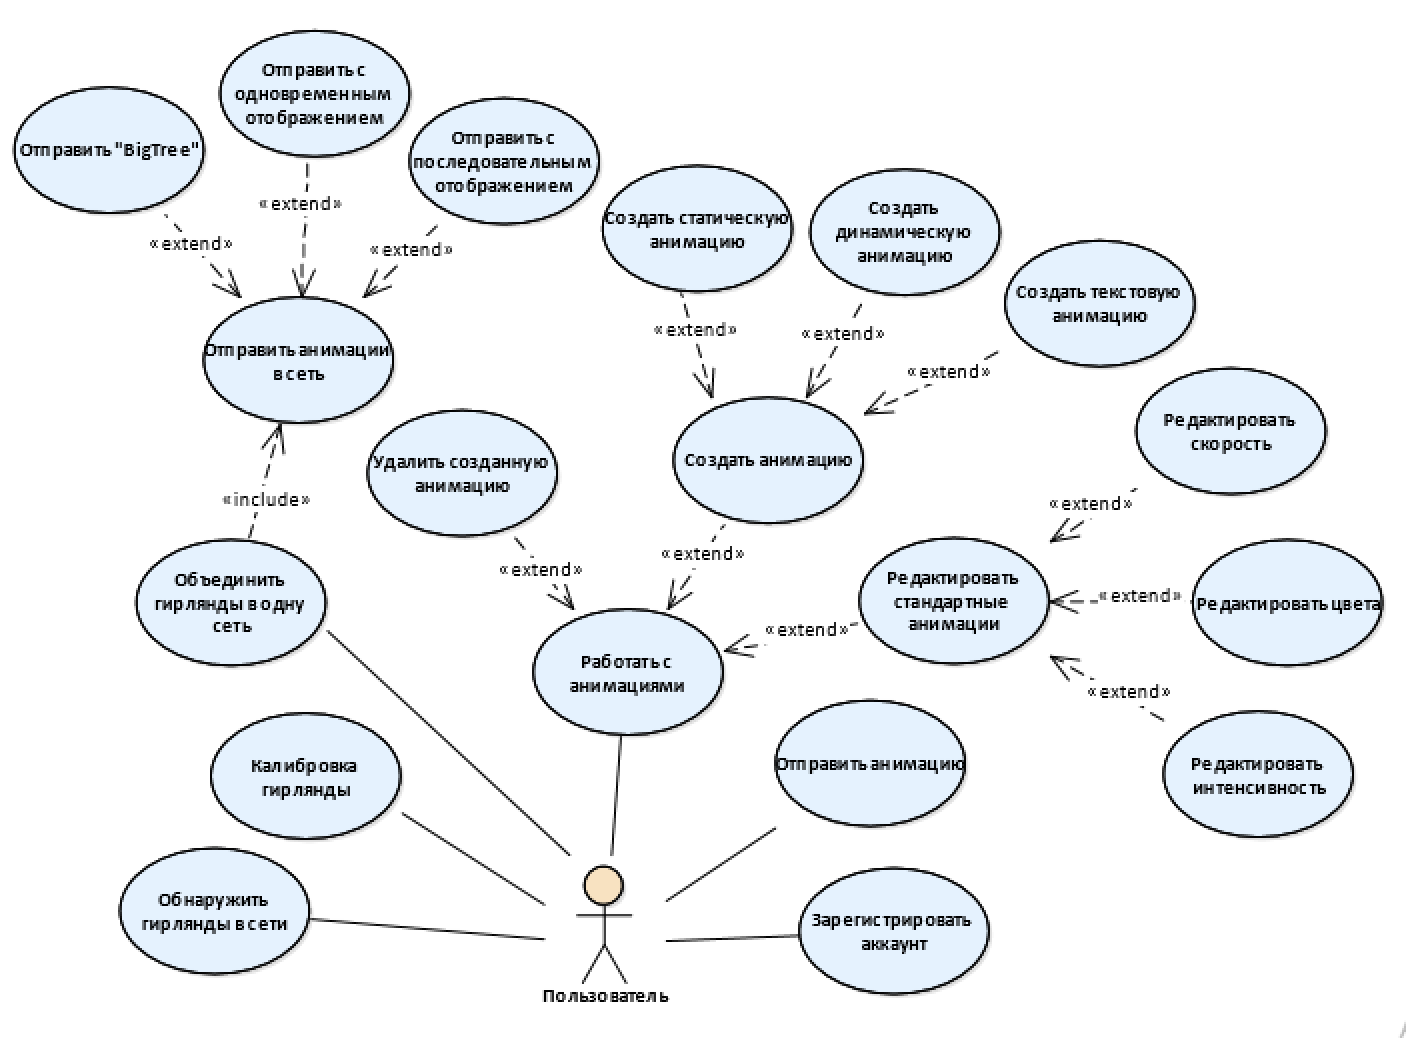
\includegraphics[scale=0.65]{figures/diagrams/uml_useCase.png}
	\caption{Диаграмма использования системы}
	\label{fig:develop:umlDiagrams:useCase}
\end{figure}

Диаграмма последовательности
% \label{sec:develop:umlDiagrams:sequence}

На диаграмме последовательностей могут присутствовать участники процесса (пользователь и адресная светодиодная лента), компоненты системы, и сообщения, которые они могут вернуть. После запуска приложения оно пытается автоматически подключится к адресной светодиодной ленте. После успешного подключения пользователь может начать редактировать стандартные анимации, постоянно перезаписывая их в базе данных. Если пользователь захочет отправить анимацию на адресную ленту, то приложение возьмет ее из базы данных, конвертирует в байты (чтобы лента могла ее воспроизвести), отчистит адресную ленту от текущей анимации на ней и отправит ее по TCP сокетам. Данная диаграмма отражена в приложении Б.

Диаграмма компонентов
% \label{sec:develop:umlDiagrams:component}

Диаграмма компонентов позволяет определить архитектуру разрабатываемой системы, установив зависимости между программными компонентами, в роли которых может выступать исходный  и исполняемый код. Диаграмму можно увидеть на рисунке~\ref{fig:develop:umlDiagrams:component}.

~
\begin{figure}[H]
\centering
	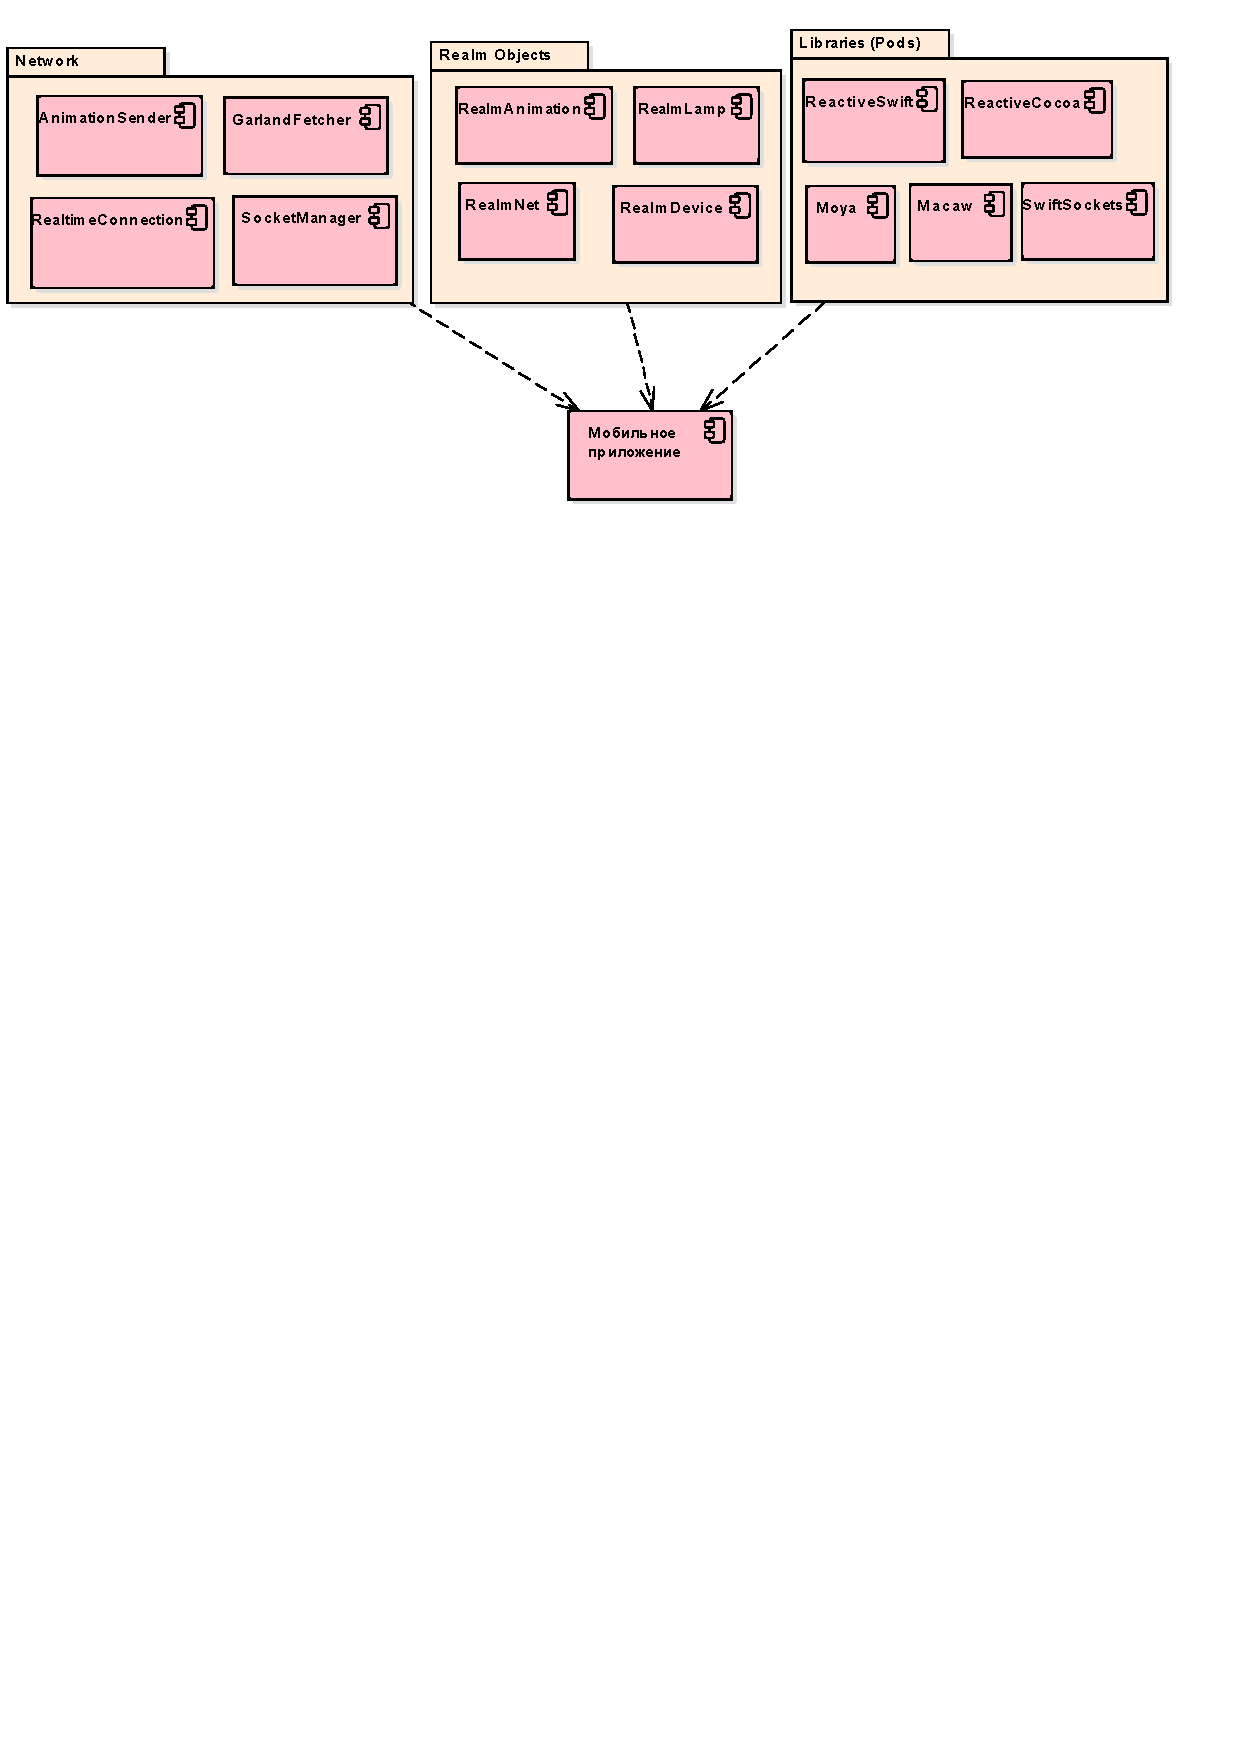
\includegraphics[scale=0.8]{figures/diagrams/uml_component.pdf}
	\caption{Диаграмма компонентов системы для управления световым оборудованием}
	\label{fig:develop:umlDiagrams:component}
\end{figure}

Диаграмма развертывания
% \label{sec:develop:umlDiagrams:deployment}

Диаграмма развертывания необходима для представления того, какие устройства будут использовать те или иные компоненты. Из диаграммы понятно, что для использования данного продукта, пользователь должен иметь мобильный телефон под управлением операционной системы iOS (iPhone), а также адресную светодиодную ленту. Для использования сетевых функций (через Firebase) нужно стабильное подключение к интернету (Рисунок~\ref{fig:develop:umlDiagrams:deployment}).

~
\begin{figure}[H]
\centering
	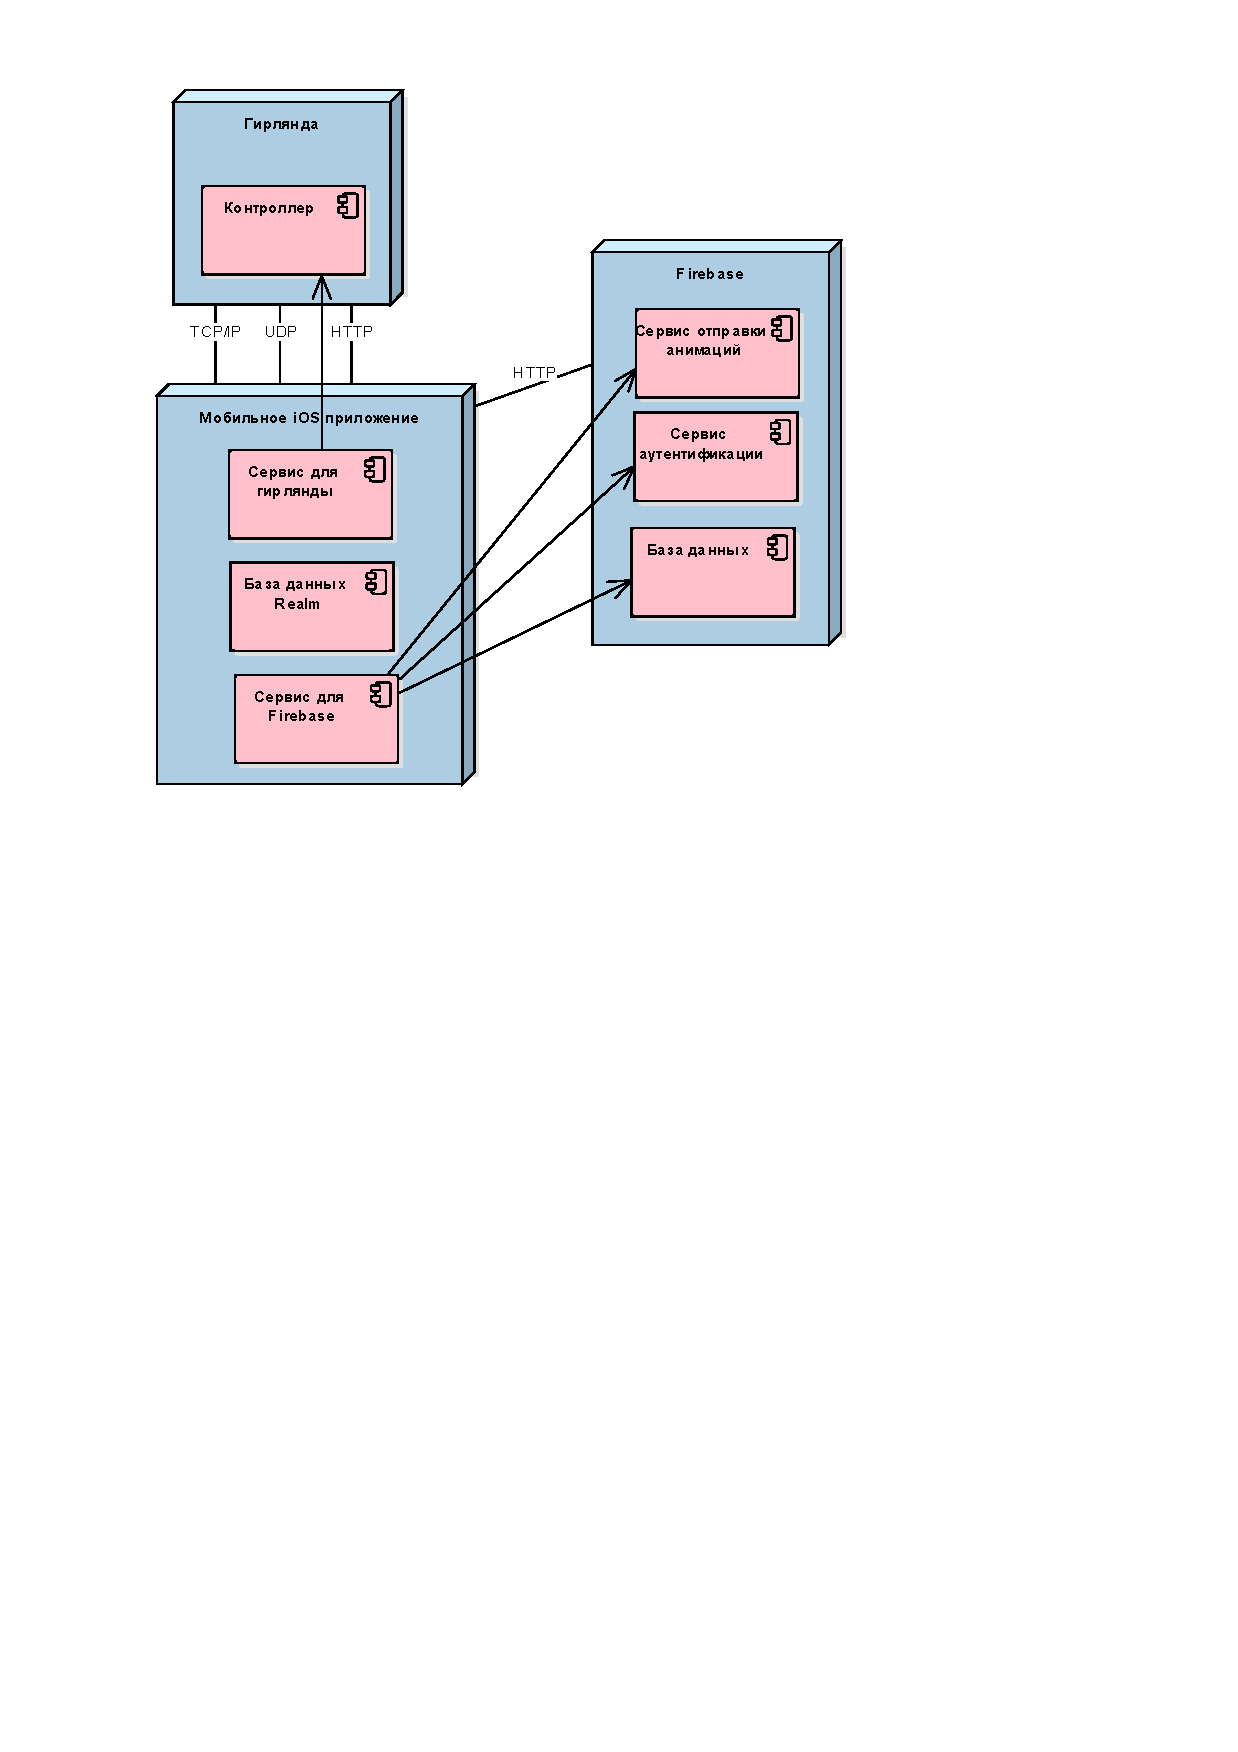
\includegraphics[scale=0.8]{figures/diagrams/uml_deployment.pdf}
	\caption{Диаграмма системы для управления световым оборудованием}
	\label{fig:develop:umlDiagrams:deployment}
\end{figure}

Диаграмма состояний
% \label{sec:develop:umlDiagrams:useCase}

Диаграмма состояний описывает все возможные состояния процесса отправки анимации. На данной диаграмме показаны все возможные состояния, которые может принимать анимация. Если адресная светодиодная лента многоканальная, то перед отправкой ее надо расширить на нужное количество лампочек. При отправке анимации сначала посылается ее полное время проигрывания, потом адресная лента отчищается от уже воспроизводимой анимации, после идет конвертация данных анимации в байты и их последующая отправка по сокетам (Рисунок~\ref{fig:develop:umlDiagrams:state}).

~
\begin{figure}[H]
\centering
	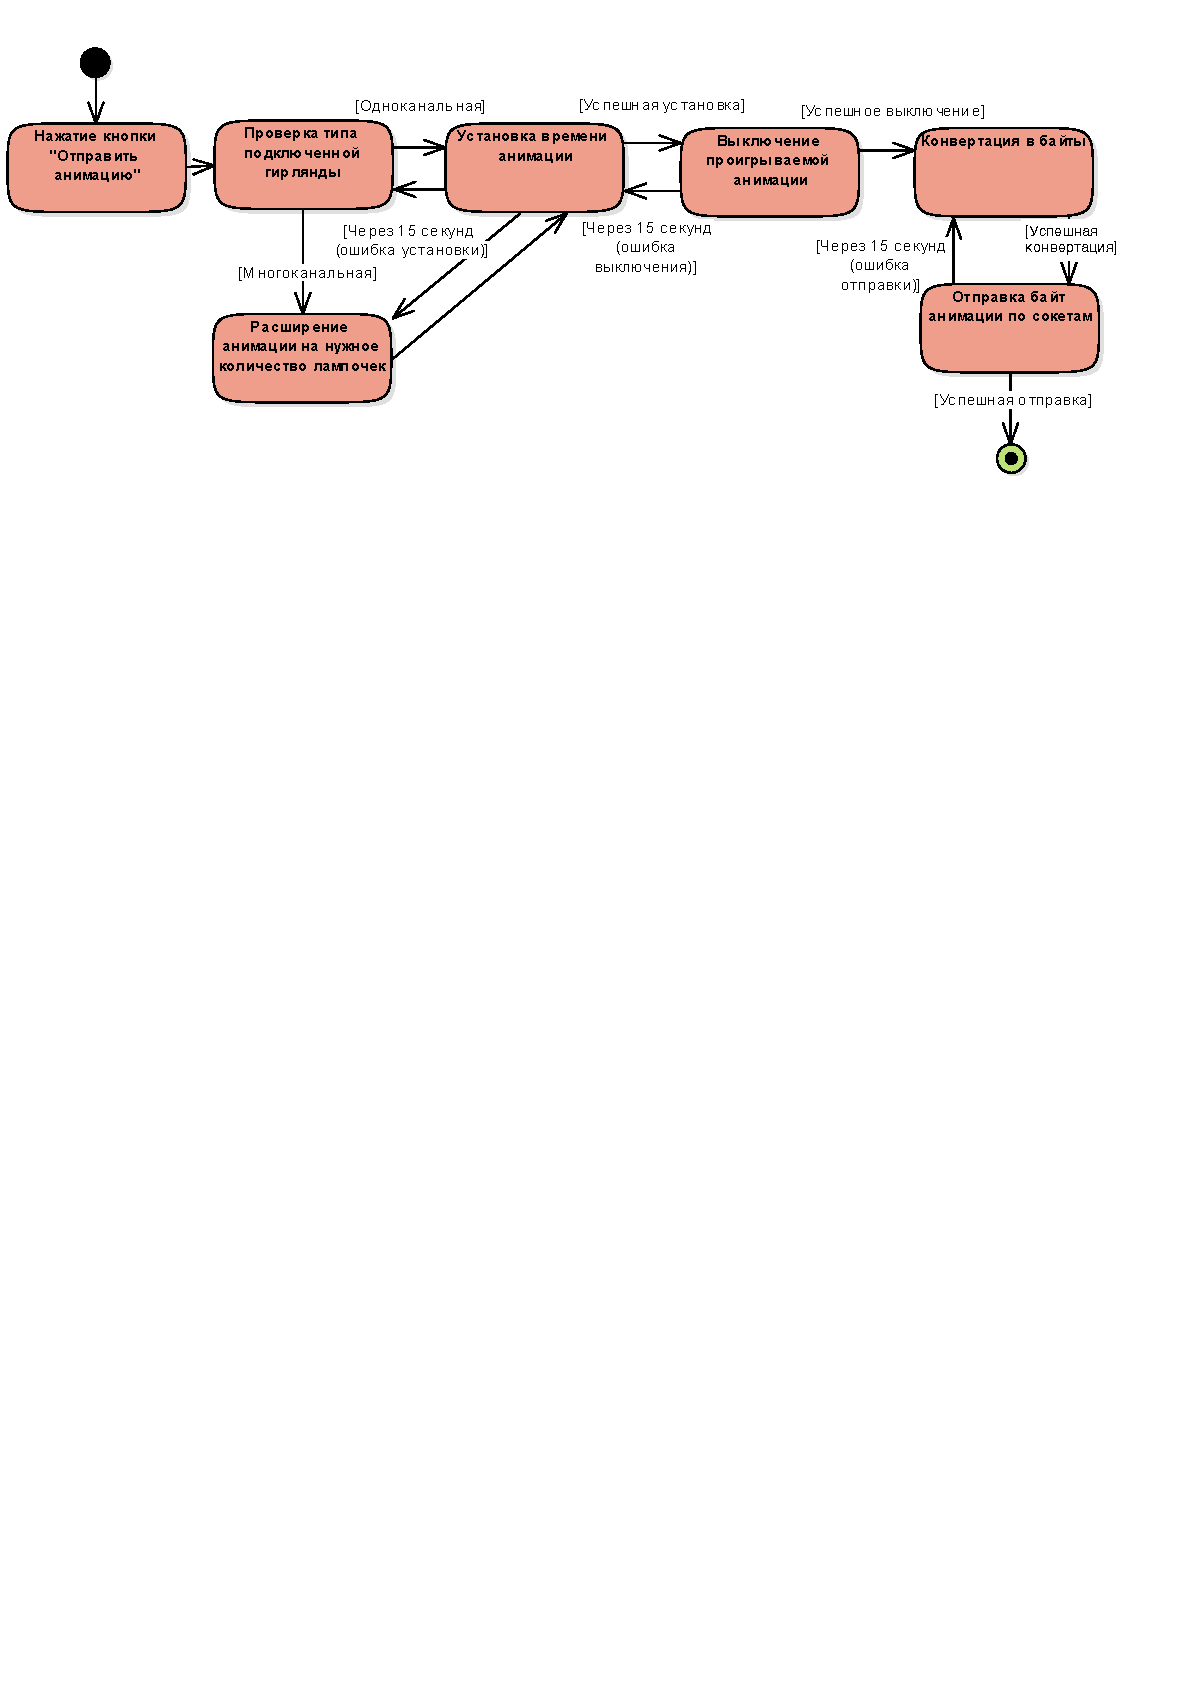
\includegraphics[scale=0.9]{figures/diagrams/uml_state.pdf}
	\caption{Диаграмма состояний анимации}
	\label{fig:develop:umlDiagrams:state}
\end{figure}

Диаграмма классов
% \label{sec:develop:umlDiagrams:class}

Диаграмма классов используется для визуального изображения отношений между классами и интерфейсами в программе. Основными классами в данном проекте являются анимации, сервисы для работы с адресными светодиодными лентами, так же используются классы, реализующие паттерн MVC, контроллеры отображения и модели представления системы (view controllers, view models). В приложении А изображена диаграмма классов приложения.


\newpage
\subsection{Описание алгоритмов работы подсистемы}
\label{sec:develop:algorithms}

\subsubsection{} Алгоритм аппроксимации
\label{sec:develop:algorithms:approximation}

При выполнении калибровки гирлянды, после обработки изображения и группировки лампочек, происходит важный этап~--- аппроксимация. Так как алгоритм не находит 100\% лампочек, но пользователю нужно анимацию на всех, то применяется данный алгоритм. Он находит участки не найденных лампочек и выстраивает прямую между двумя крайними найденными лампочками. И на данную прямую равномерно наносятся не найденные лампочки. Алгоритм представлен в приложении Г на рисунке Г.1.

\subsubsection{} Алгоритм конвертации байт анимации
\label{sec:develop:algorithms:bytesSending}

При отправке анимации на гирлянду происходит ее конвертация в байты для оптимизации как самого процесса отправки (уменьшая ее время), так и процесс отображения анимации на гирлянде, правильно компонуя байты лампочек друг с другом. В самом алгоритме лампочки сортируются по кадрам анимации (по deltaT) и разбиваются на порции по 50 лампочек, после этого они конвертируются в байты, группируются и отправляются на гирлянду. Данный алгоритм представлен в приложении Г на рисунке Г.2.

\newpage
\subsection{Информационная модель системы}
\label{sec:develop:umlDiagrams}

Чтобы разработать мобильное приложение для управления адресной светодиодной лентой необходимо представить информационную модель этой системы. Система рассмотрена в виде совокупности объектов и связей между ними. 

Представления информационной модели в графическом виде (логический и физический уровни) приведены на диаграмме В.1 и В.2 приложения В. Модель приведена к третьей нормальной форме.

При проектировании системы для поиска, вызова и оплаты такси были выделены такие сущности, как:
\begin{itemize}
	\item Анимация;
	\item Лампочка;
	\item Отображение;
	\item Сеть;
	\item Устройство (гирлянда);
	\item Пользователь.
\end{itemize}

Сущность Анимация необходима для отображения стандартных и пользовательских анимаций в приложении и содержит в себе следующие атрибуты:
\begin{itemize}
	\item name~-- имя анимации;
	\item animation\_id~-- id анимации, используется при отправке анимации на гирлянду (0~-- посылается через байты, 1, 2,...~-- запускает анимацию внутри самой гирлянды);
	\item previewType~-- тип анимации (default, custom);
	\item totalTime~-- полное время анимации;
	\item speed~-- скорость анимации;
	\item type~-- тип отображения в приложении (string, tree, custom, grid);
	\item createdDate~-- дата создания;
	\item currentColorIndex~-- выбранный набор цветов;
	\item maximumColorsCount~-- максимальное количество цветов в наборе;
	\item maximumSpeed~-- максимальное значение скорости;
	\item minimumSpeed~-- минимальное значение скорости;
	\item intensity~-- интенсивность анимации;
	\item editOptions~-- доступные опции для редактирования;
	\item colors~-- наборы цветов.
\end{itemize}

Сущность Лампочка необходима для представления лампочки на гирлянде под определенным адресом в конкретный момент времени и содержит в себе следующие атрибуты:
\begin{itemize}
	\item lamps\_id~-- id лампочки;
	\item address~-- адрес лампочки;
	\item color~-- цвет лампы;
	\item coordX~-- координата по оси абсцисс;
	\item coordY~-- координата по оси ординат;
	\item deltaT~-- момент времени, когда лампочка должна загореться;
	\item animation\_id~-- id анимации, к которой принадлежит лампочка;
	\item preview\_id~-- id отображения, к которому принадлежит лампочка.
\end{itemize}

Сущность Отображение необходима для представления гирлянды на экране приложения и содержит в себе следующие атрибуты:
\begin{itemize}
	\item preview\_id~-- id отображения;
	\item name~-- имя отображения;
	\item totalTime;
	\item type~-- тип отображения;
	\item lamps~-- лампочки отображения.
\end{itemize}

Сущность Сеть необходима для представления сети из гирлянд и содержит в себе следующие атрибуты:
\begin{itemize}
	\item net\_id~-- id сети;
	\item name~-- имя сети;
	\item animationName~-- имя анимации, проигрываемой на сети;
	\item animationState~-- тип отображения анимаций в сети;
	\item devices~-- устройства в сети.
\end{itemize}

Сущность Устройство необходима для представления гирлянды в сети и содержит в себе следующие атрибуты:
\begin{itemize}
	\item device\_id~-- id устройства;
	\item name~-- имя устройства;
	\item ip~-- ip-адрес устройства;
	\item port~-- порт в сети;
	\item mac~-- mac-адрес устройства;
	\item animationName~-- проигрываимая анимация на устройстве;
	\item lampsType~-- тип лампочек на устройстве;
	\item isChosen~-- флаг выбрано ли устройство для анимирования в сети;
	\item net\_id~-- id сети, к которому принадлежит устройство.
\end{itemize}

Сущность Пользователь необходима для представления пользователя для отправки анимаций и содержит в себе следующие атрибуты:
\begin{itemize}
	\item phoneNumber~-- номер телефона пользователя;
	\item email~-- email-адрес пользователя.
\end{itemize}

\newpage
\subsection{Руководство пользователя}
\label{sec:develop:userGuide}

Первое что увидит пользователь при открытии приложения~--- экран подключения к гирлянде (Рисунок~\ref{fig:develop:userGuide:loading}). Если приложение не смогло загрузить список гирлянд в сети (Рисунок), или подключиться к гирлянде напрямую, то показывается экран с возможностью попробовать еще раз (Рисунок~\ref{fig:develop:userGuide:failedLoading}), либо пропустить этот шаг и сразу перейти на главный экран приложения (Рисунок~\ref{fig:develop:userGuide:mainTree}).

~
\begin{figure}[H]
\centering
	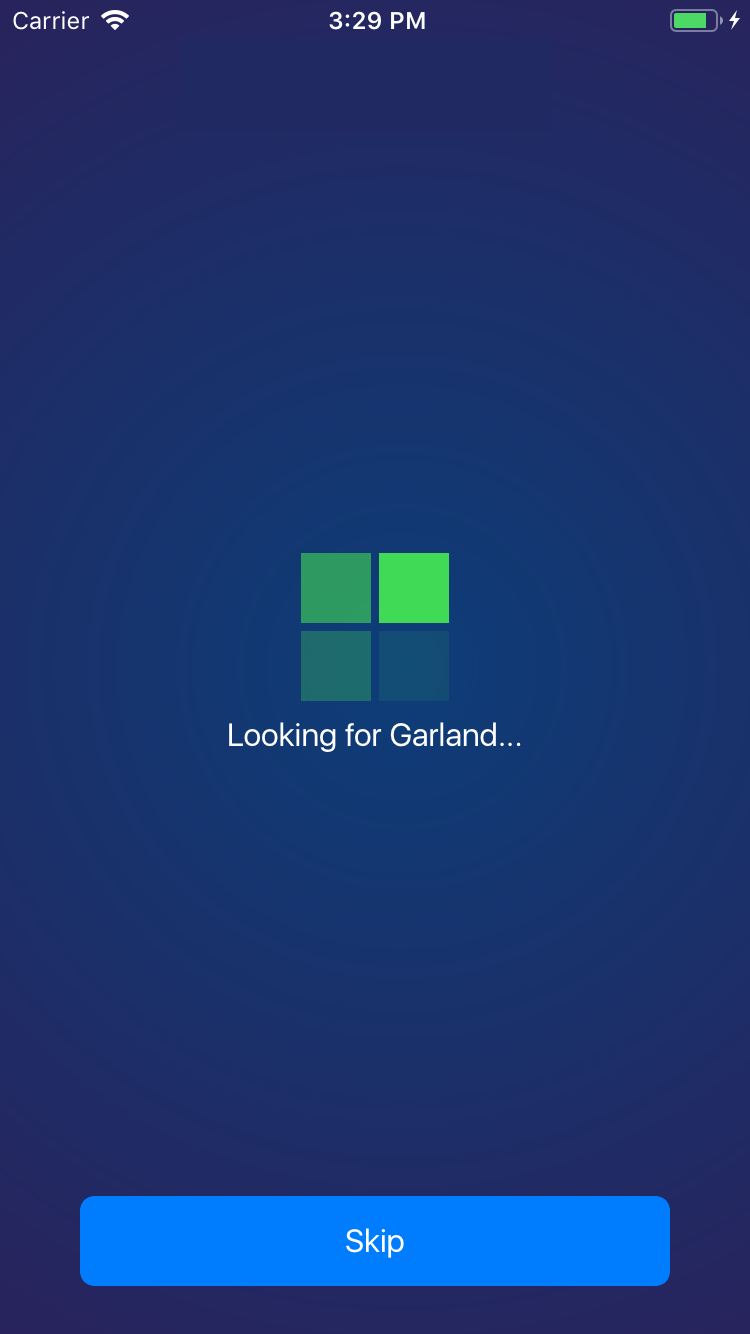
\includegraphics[scale=0.25]{figures/userGuide/loading.png}
	\caption{Экран подключения к гирлянде}
	\label{fig:develop:userGuide:loading}
\end{figure}
~
\begin{figure}[H]
\centering
	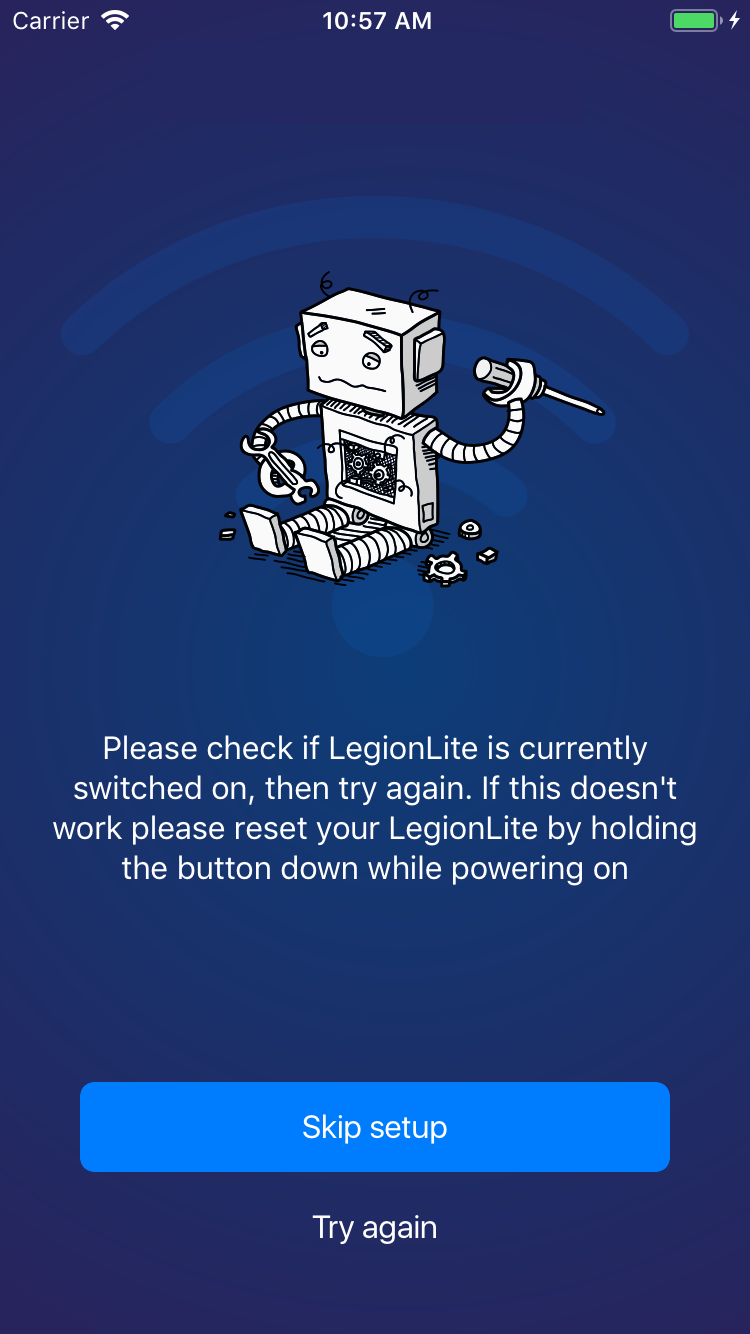
\includegraphics[scale=0.2]{figures/userGuide/failedLoading.png}
	\caption{Экран ошибки подключения к гирлянде}
	\label{fig:develop:userGuide:failedLoading}
\end{figure}
~
\begin{figure}[H]
\centering
	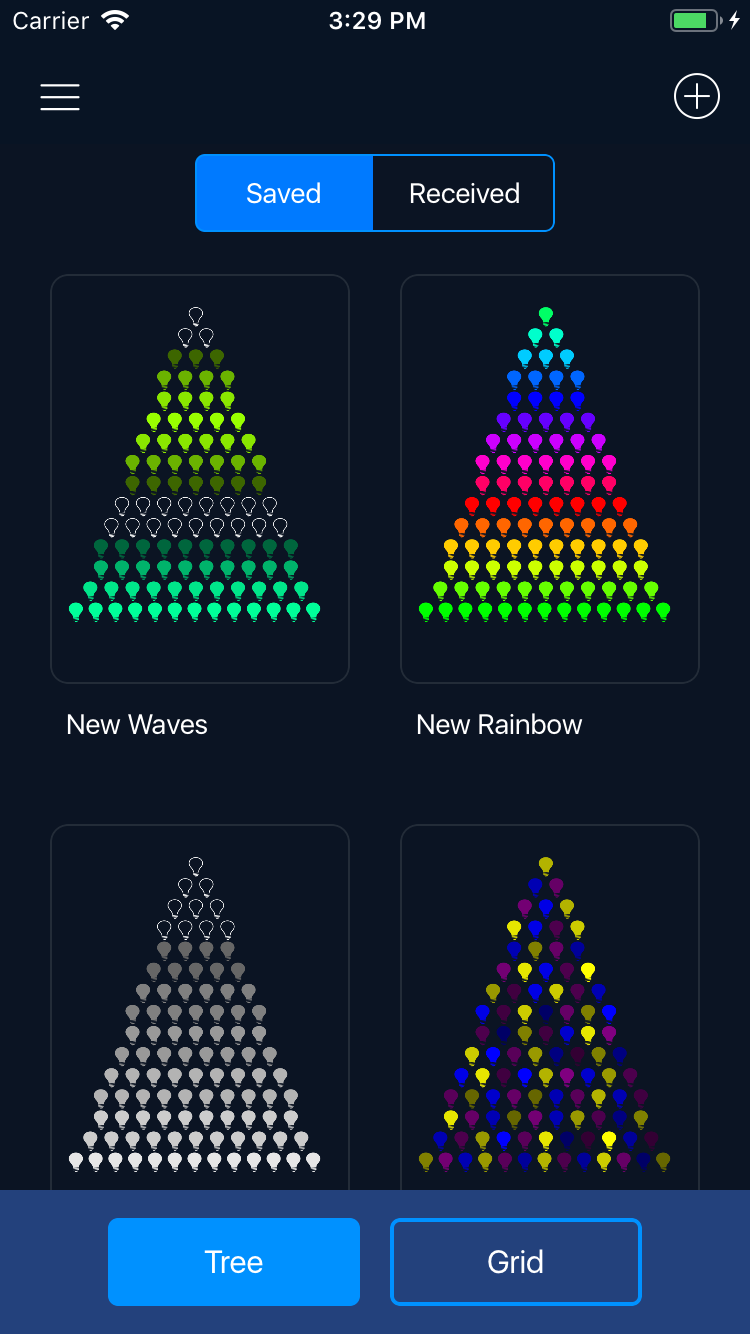
\includegraphics[scale=0.2]{figures/userGuide/mainTree.png}
	\caption{Список всех доступных анимаций для гирлянд типа ``дерево''}
	\label{fig:develop:userGuide:mainTree}
\end{figure}

На главном экране приложения (список всех доступных анимаций), пользователь может выбрать типы просматриваемых доступных анимаций (либо ``Tree'' на рисунке~\ref{fig:develop:userGuide:mainTree}, либо ``Grid'', рисунок~\ref{fig:develop:userGuide:mainGrid}), может создать собственную анимацию по нажатию на кнопку ``+'' (Рисунок~\ref{fig:develop:userGuide:drawingCustom}). Также пользователь, по нажатию на ``гамбургер'', может перейти в меню (Рисунок~\ref{fig:develop:userGuide:sideMenu}). На экране создания собственной анимации пользователь имеет несколько инструментов: точечная кисть (красит по одной лампочке за раз), толстая кисть (красит несколько лампочек за раз) и ластик. Еще пользователь может выбрать нужны цвет с помощью цветового круга (Рисунок~\ref{fig:develop:userGuide:colorPicker}).

~
\begin{figure}[H]
\centering
	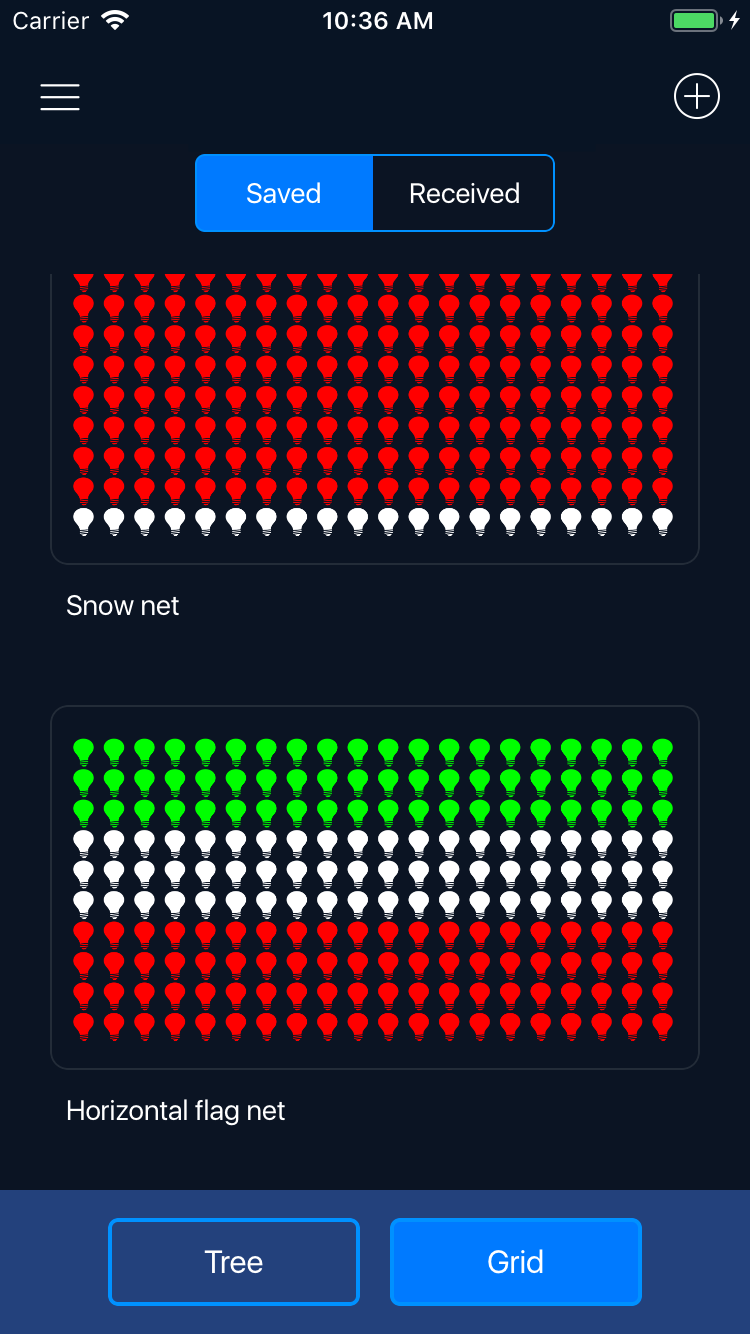
\includegraphics[scale=0.2]{figures/userGuide/mainGrid.png}
	\caption{Список всех доступных анимаций для гирлянд типа ``сетка''}
	\label{fig:develop:userGuide:mainGrid}
\end{figure}
~
\begin{figure}[H]
\centering
	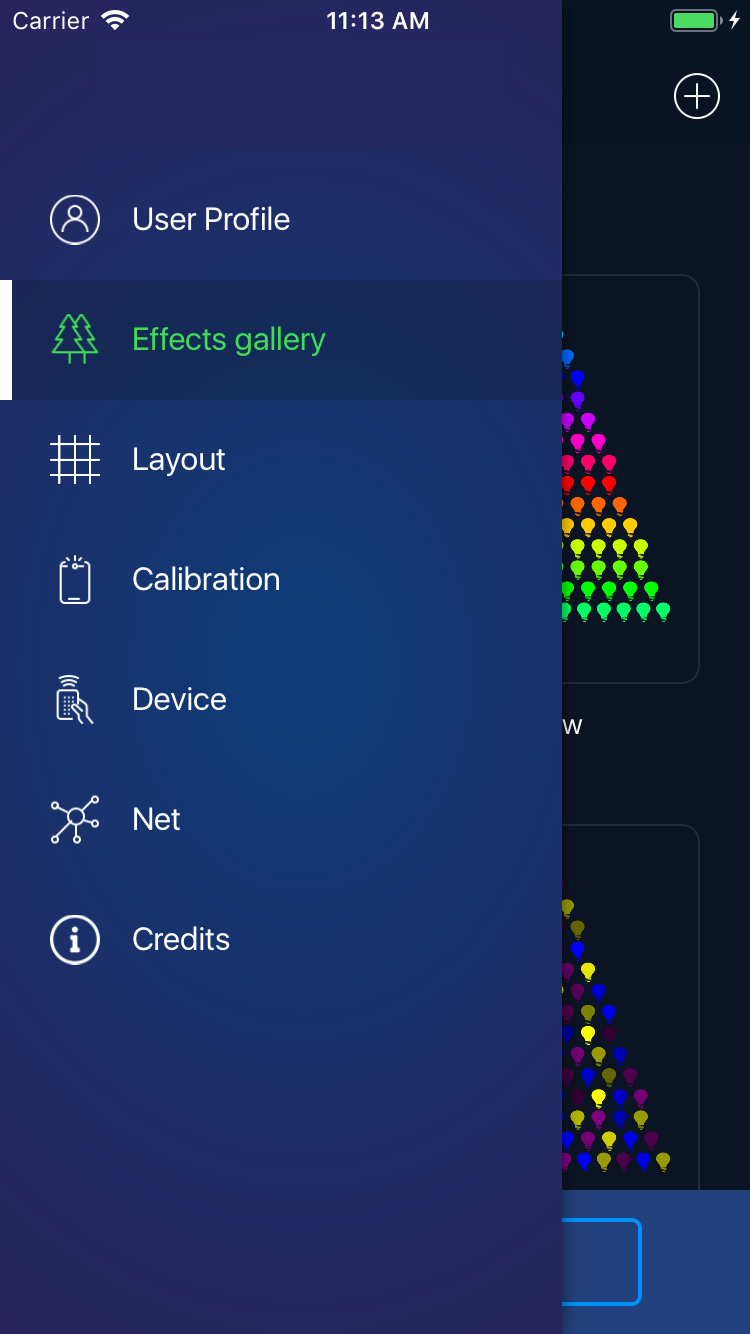
\includegraphics[scale=0.2]{figures/userGuide/sideMenu.png}
	\caption{Меню приложения}
	\label{fig:develop:userGuide:sideMenu}
\end{figure}
~
\begin{figure}[H]
\centering
	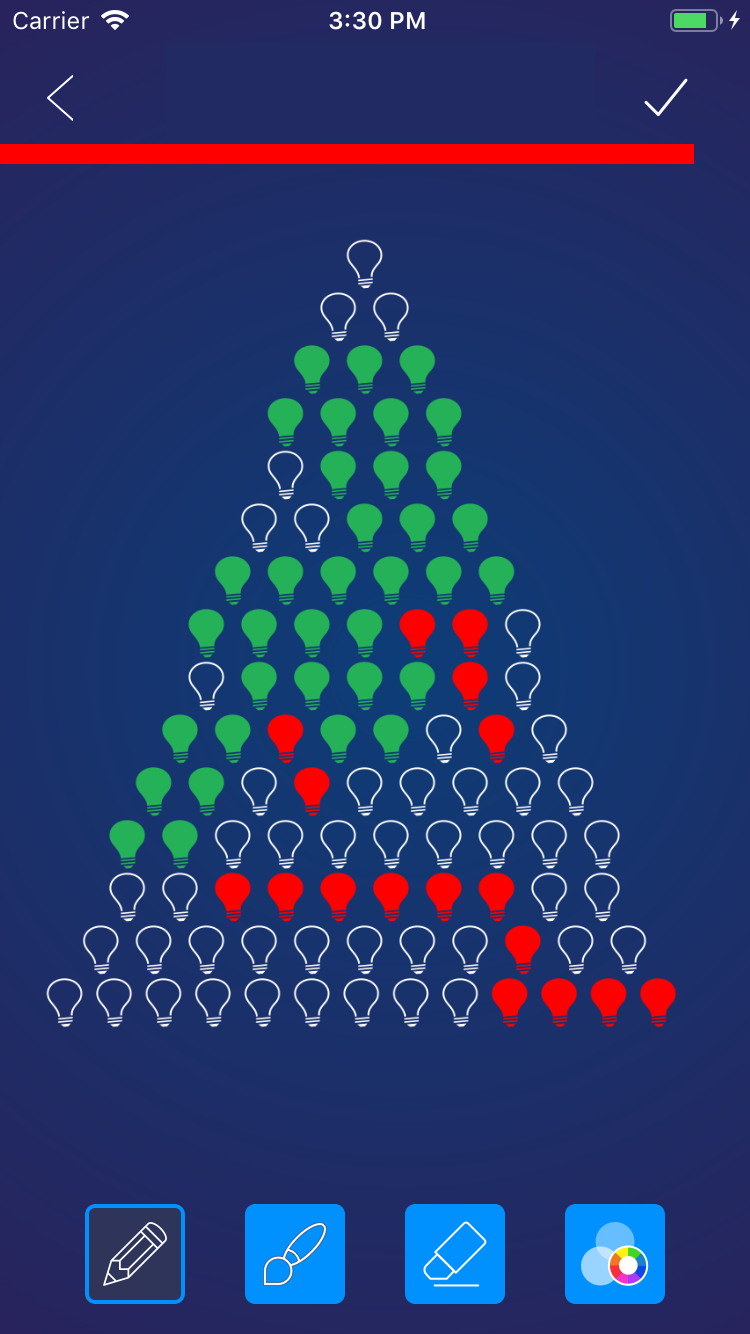
\includegraphics[scale=0.2]{figures/userGuide/drawingCustom.png}
	\caption{Экран создания собственной анимации}
	\label{fig:develop:userGuide:drawingCustom}
\end{figure}
~
\begin{figure}[H]
\centering
	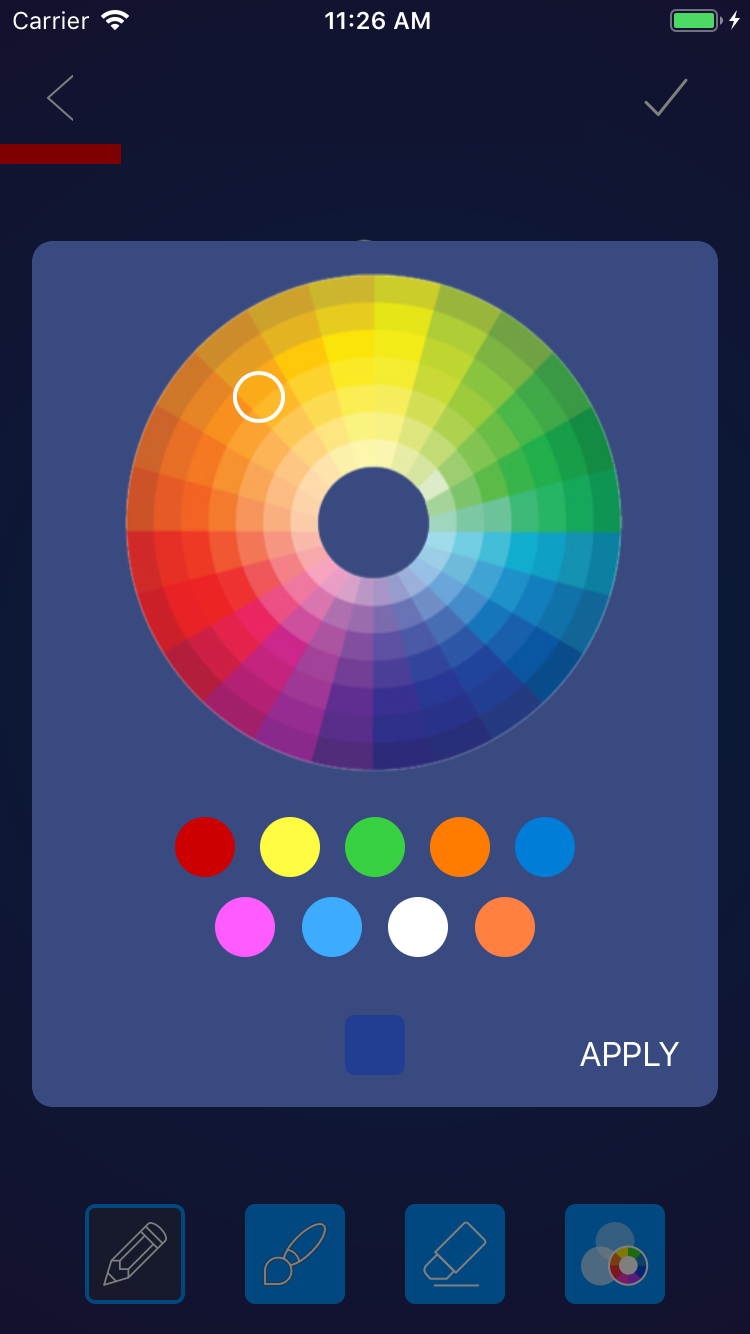
\includegraphics[scale=0.2]{figures/userGuide/colorPicker.png}
	\caption{Экран выбора цвета}
	\label{fig:develop:userGuide:colorPicker}
\end{figure}

При нажатии на анимацию из списка на главном экране, пользователь перейдет на экран просмотра данной анимации (Рисунок~\ref{fig:develop:userGuide:previewDefault}). На данном экране пользователь может отправить анимацию на гирлянду, отправить анимацию другому пользователю, используя его номер телефона (Рисунок~\ref{fig:develop:userGuide:sendingAnimation}), и перейти на экран редактирования анимации. На экране редактирования анимации пользователь, в зависимости от типа анимации может редактировать интенсивность, скорость и набор цветов у анимации (Рисунки~\ref{fig:develop:userGuide:editingNewWaves} и~\ref{fig:develop:userGuide:editingSnake}). Для формирования набора цветов пользователь должен перейти в специальный экран с цветовым кругом (Рисунок~\ref{fig:develop:userGuide:editingColorSequence}).

~
\begin{figure}[H]
\centering
	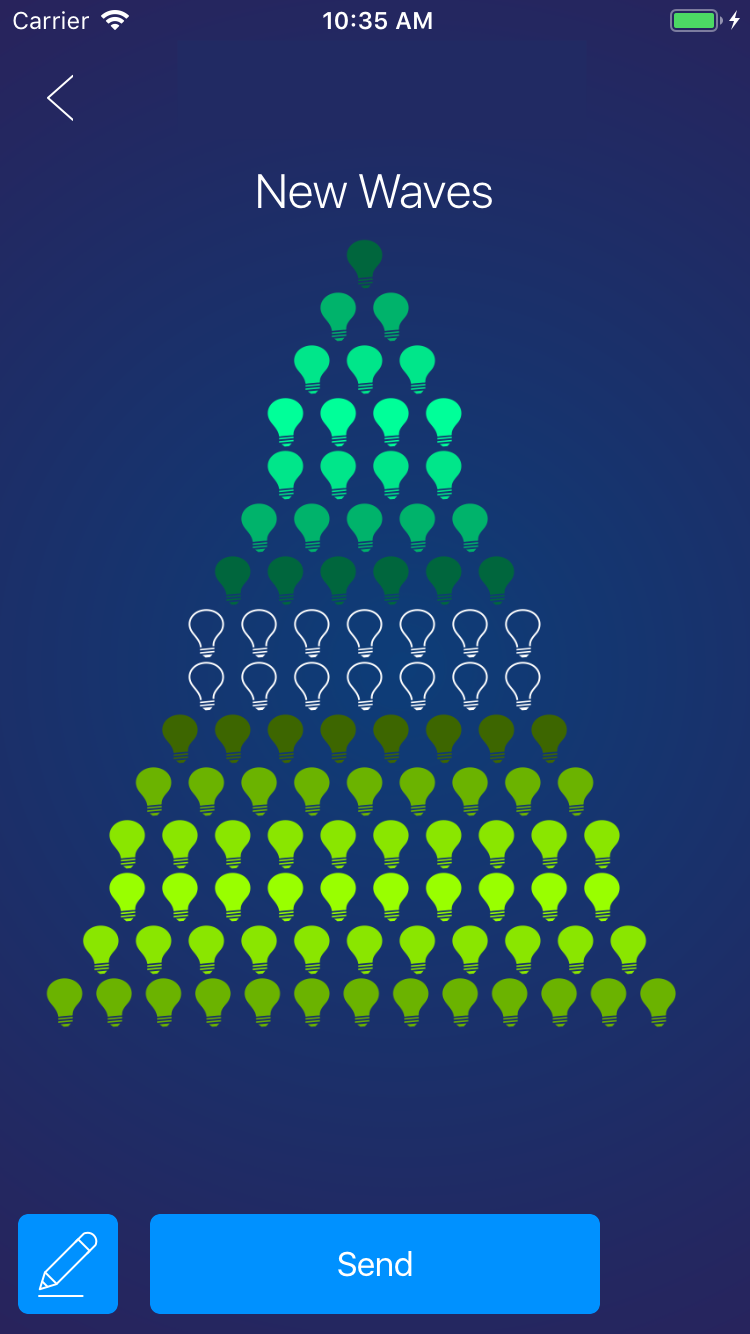
\includegraphics[scale=0.2]{figures/userGuide/previewDefault.png}
	\caption{Экран просмотра существующей анимации}
	\label{fig:develop:userGuide:previewDefault}
\end{figure}
~
\begin{figure}[H]
\centering
	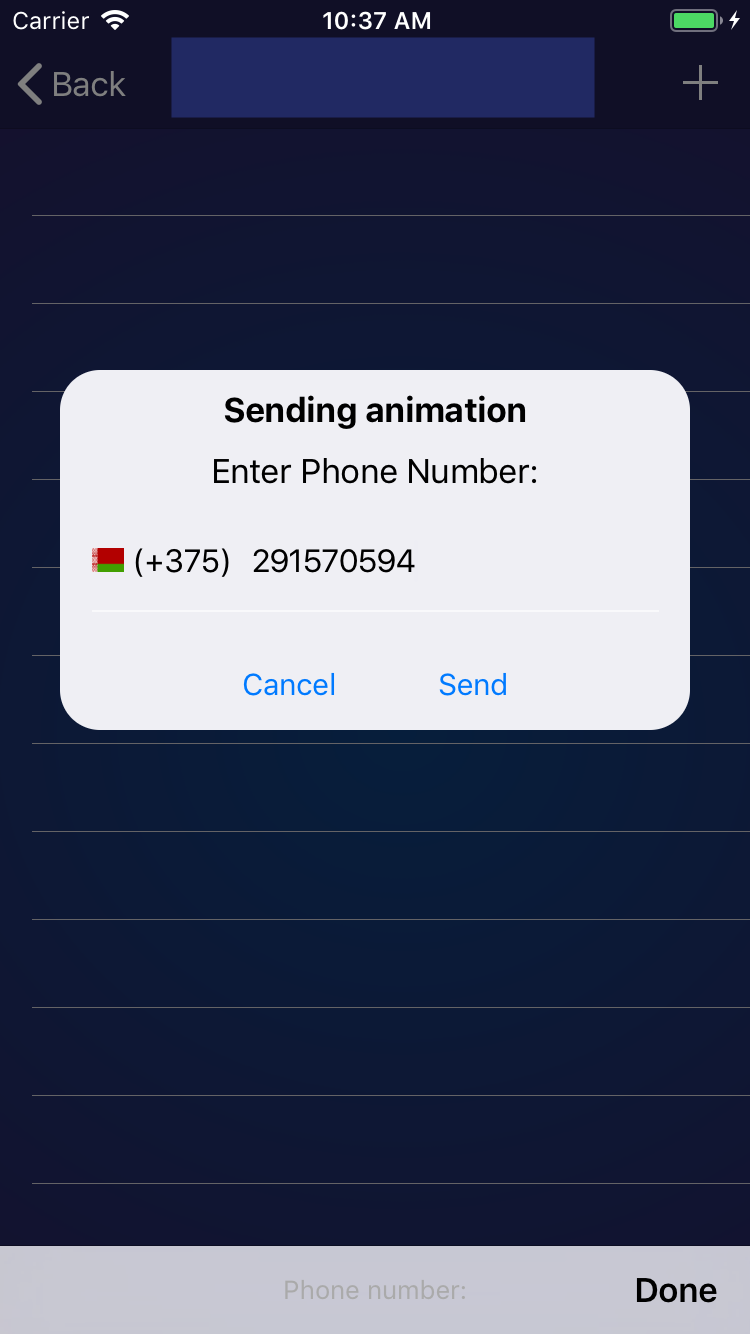
\includegraphics[scale=0.2]{figures/userGuide/sendingAnimation.png}
	\caption{Экран отправки анимации другому пользователю}
	\label{fig:develop:userGuide:sendingAnimation}
\end{figure}
~
\begin{figure}[H]
\centering
	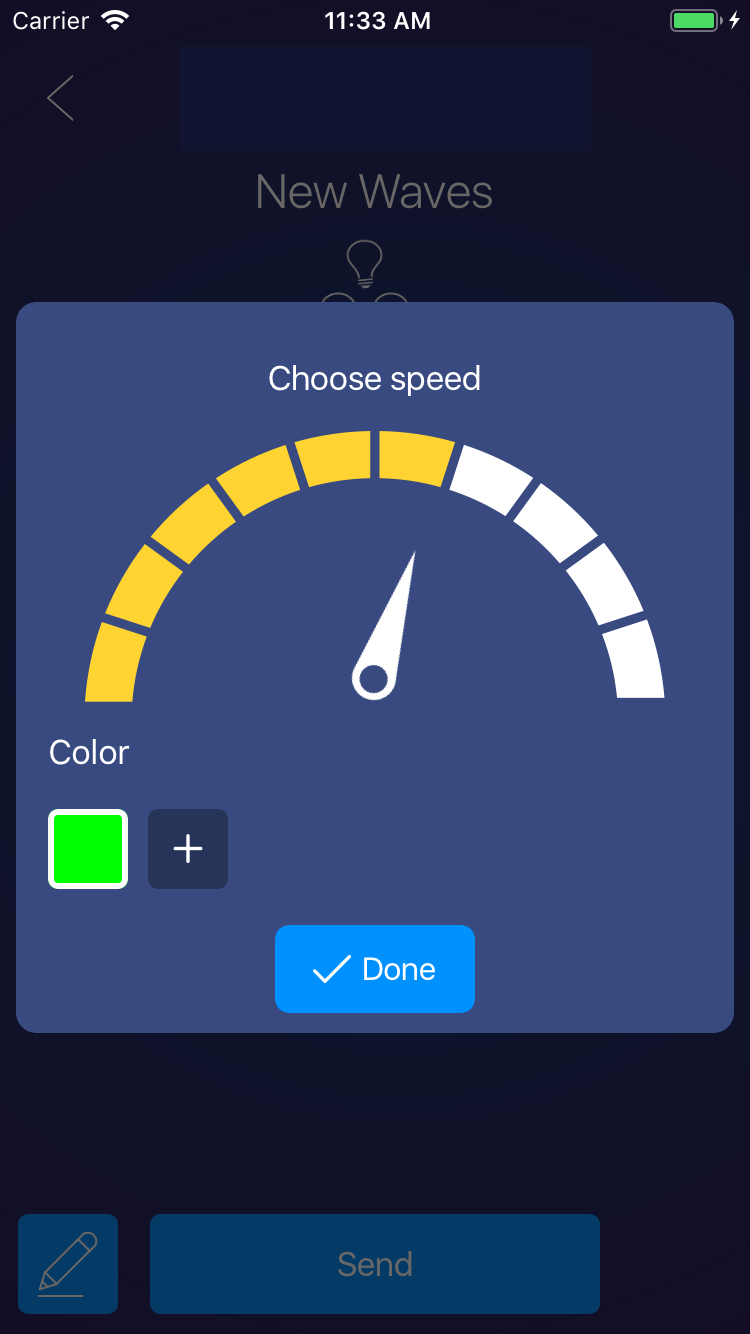
\includegraphics[scale=0.2]{figures/userGuide/editingNewWaves.png}
	\caption{Экран редактирования анимации ``New Waves''}
	\label{fig:develop:userGuide:editingNewWaves}
\end{figure}
~
\begin{figure}[H]
\centering
	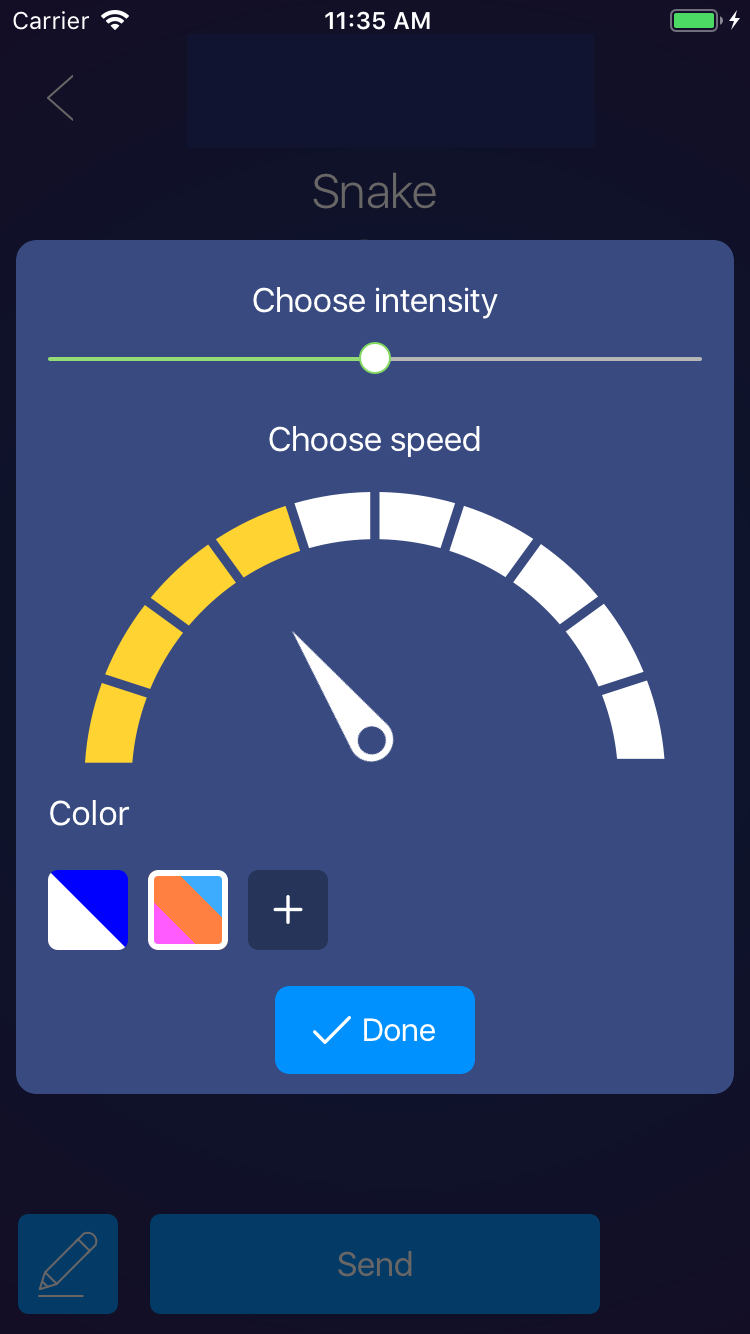
\includegraphics[scale=0.2]{figures/userGuide/editingSnake.png}
	\caption{Экран редактирования анимации ``Snake''}
	\label{fig:develop:userGuide:editingSnake}
\end{figure}
~
\begin{figure}[H]
\centering
	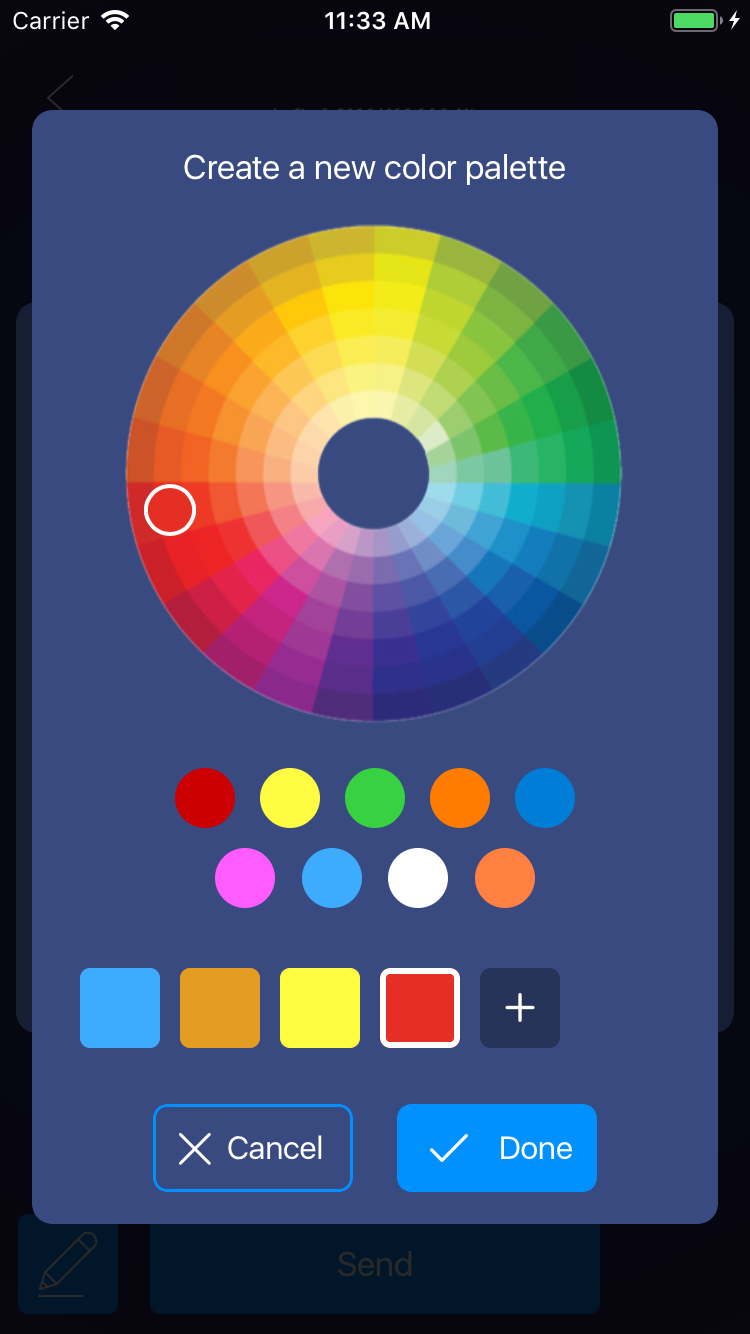
\includegraphics[scale=0.2]{figures/userGuide/editingColorSequence.png}
	\caption{Экран выбора последовательности цветов}
	\label{fig:develop:userGuide:editingColorSequence}
\end{figure}

Чтобы отправить анимацию другому человеку, пользователь должен зайти в свой аккаунт в приложении (Рисунок~\ref{fig:develop:userGuide:signIn}), либо, если у него его еще нет, то зарегистрироваться используя свой номер телефона, электронную почту и пароль (Рисунок~\ref{fig:develop:userGuide:signUp}).

~
\begin{figure}[H]
\centering
	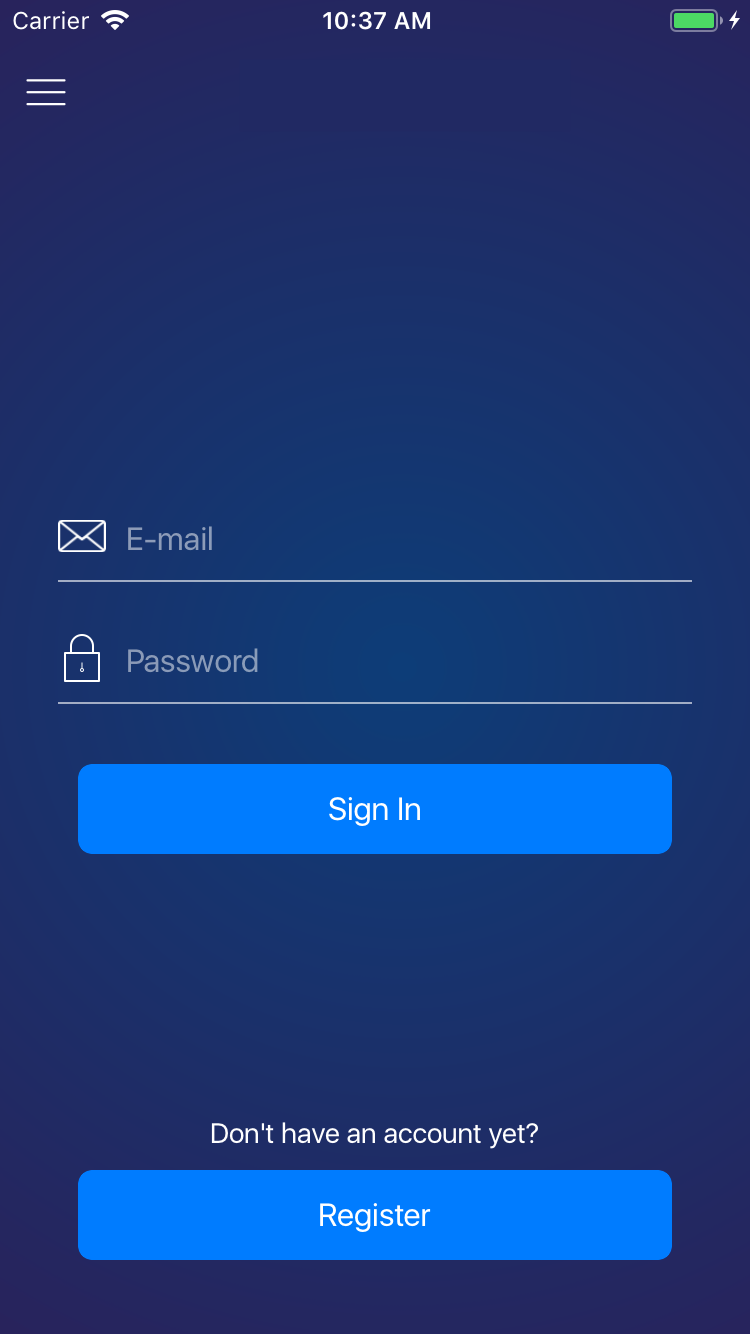
\includegraphics[scale=0.2]{figures/userGuide/signIn.png}
	\caption{Экран входа в аккаунт}
	\label{fig:develop:userGuide:signIn}
\end{figure}
~
\begin{figure}[H]
\centering
	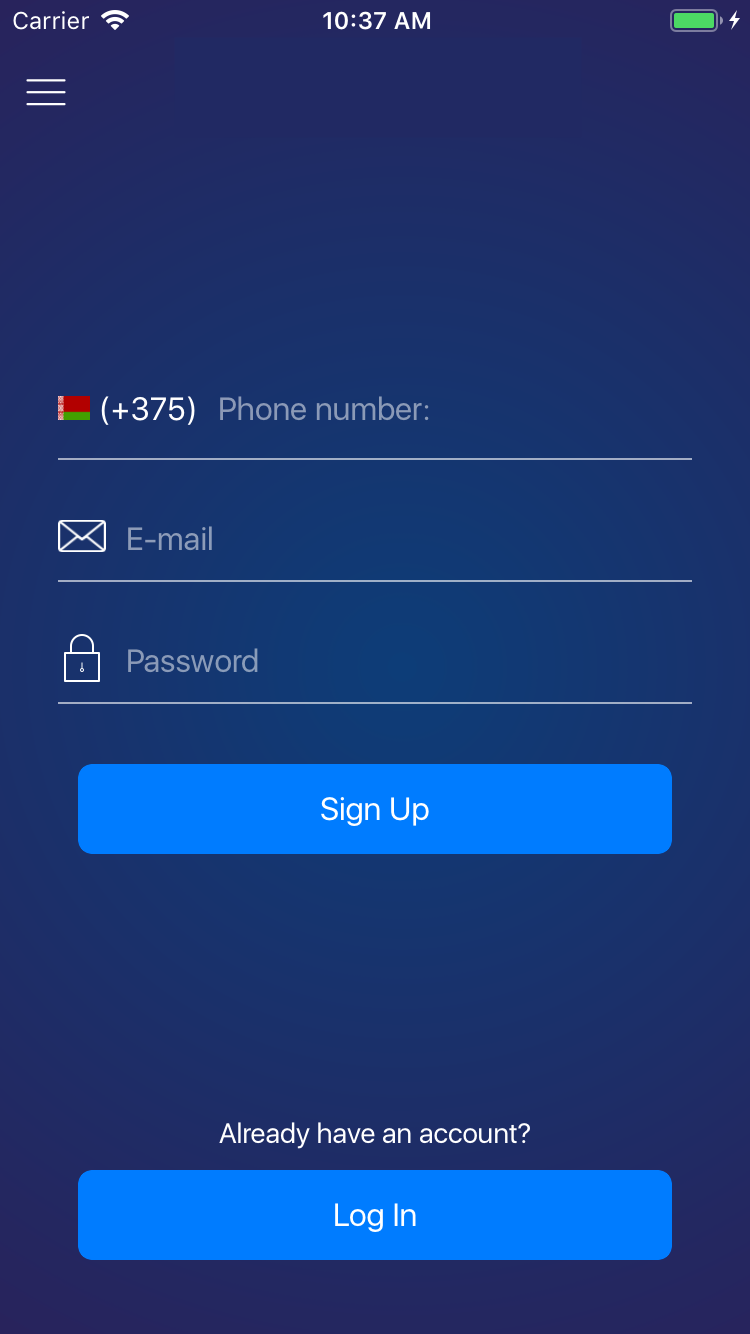
\includegraphics[scale=0.2]{figures/userGuide/signUp.png}
	\caption{Экран регистрации}
	\label{fig:develop:userGuide:signUp}
\end{figure}

Если пользователь подключен к гирлянде напрямую (подключился к ней, как к Wi-Fi точке), то экран ``Устройство'' выглядит как на рисунке~\ref{fig:develop:userGuide:device}. На нем пользователь может подключить ее к существующему Wi-Fi роутеру и просмотреть информацию о гирлянде (ip, mac адреса, версию прошивки, имя гирлянды и т.д.) (Рисунок~\ref{fig:develop:userGuide:device}). Если же пользователь подключен к роутеру, то он будет видеть список доступных гирлянд в этой сети (Рисунок~\ref{fig:develop:userGuide:device}).

~
\begin{figure}[H]
\centering
	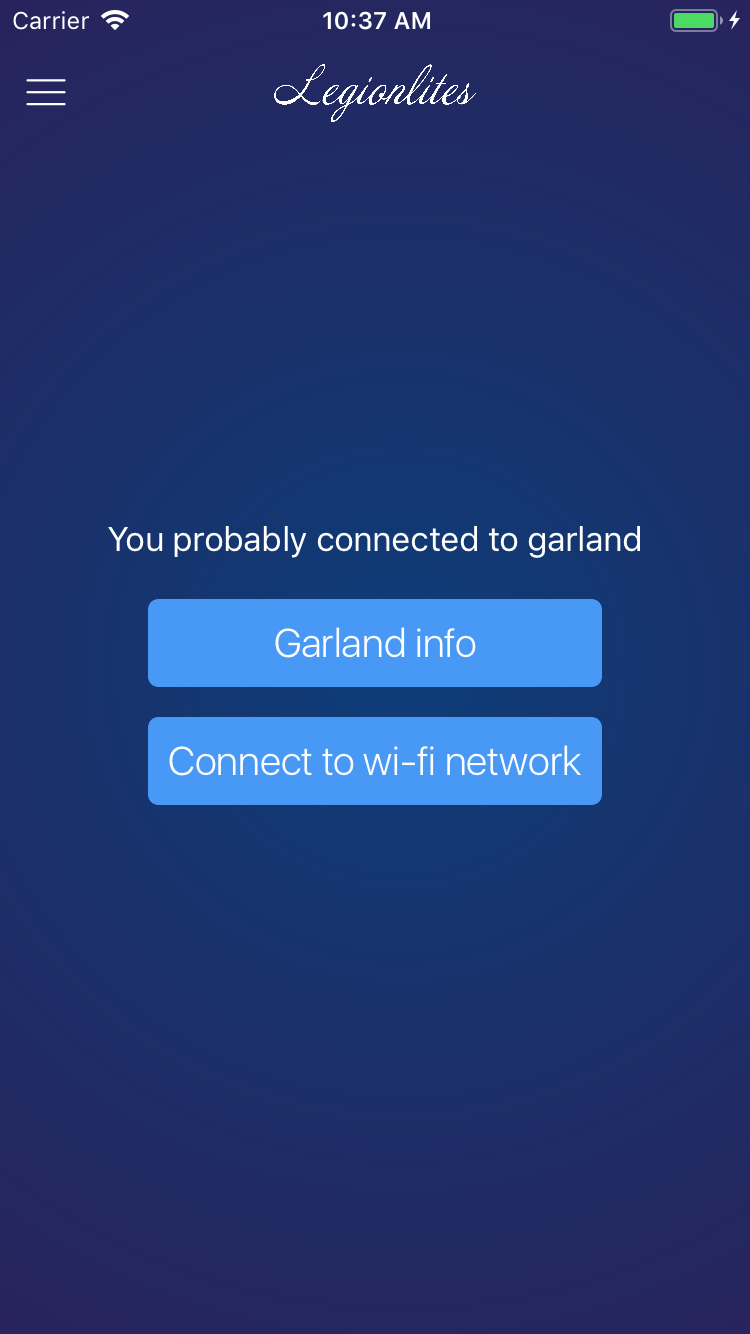
\includegraphics[scale=0.2]{figures/userGuide/device.png}
	\caption{Экран регистрации}
	\label{fig:develop:userGuide:device}
\end{figure}
~
\begin{figure}[H]
\centering
	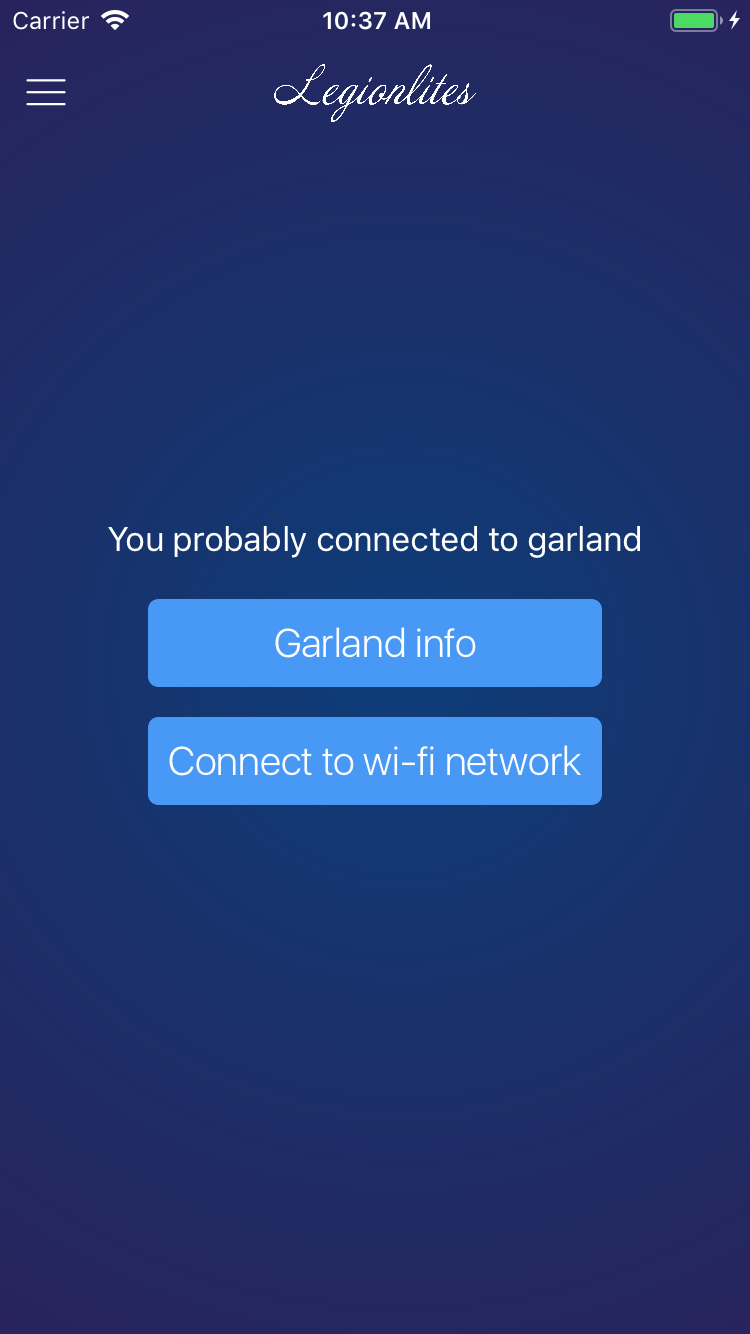
\includegraphics[scale=0.2]{figures/userGuide/device.png}
	\caption{Экран регистрации}
	\label{fig:develop:userGuide:device}
\end{figure}
~
\begin{figure}[H]
\centering
	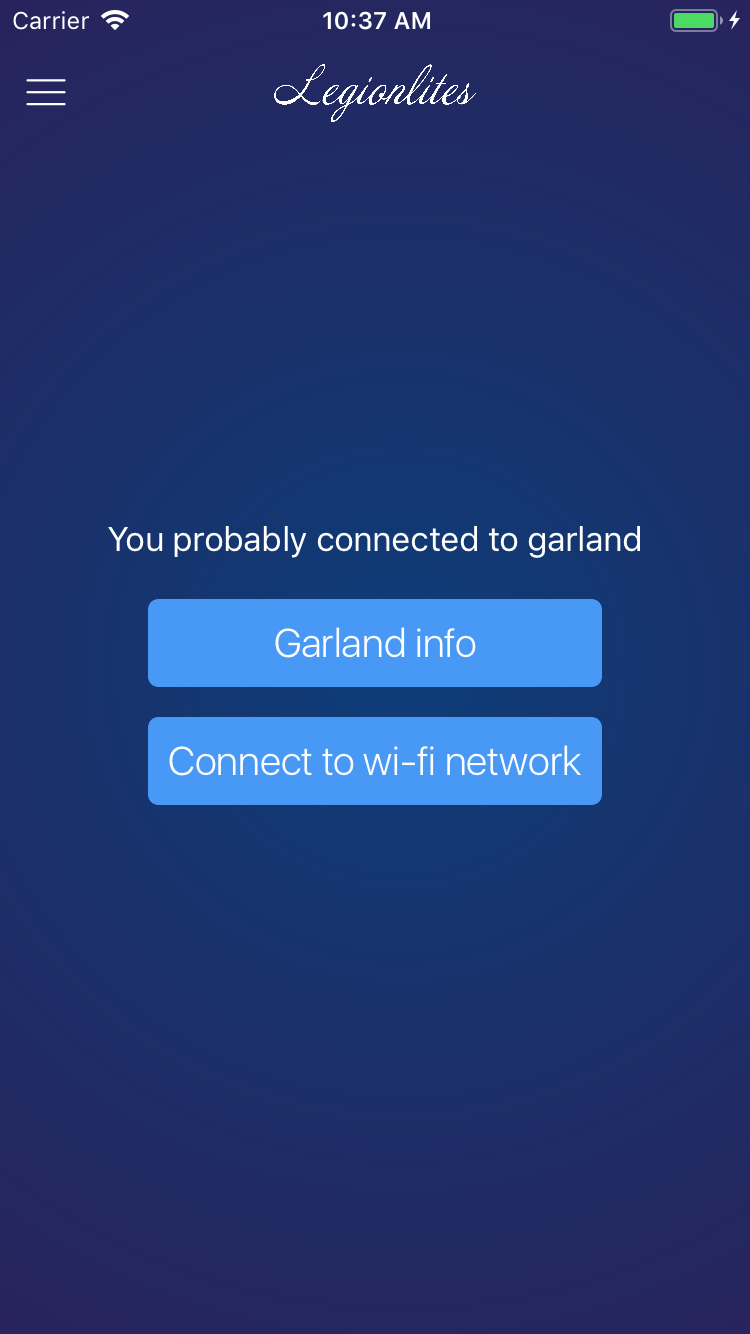
\includegraphics[scale=0.2]{figures/userGuide/device.png}
	\caption{Экран регистрации}
	\label{fig:develop:userGuide:device}
\end{figure}

Для завершения работы с гирляндой пользователю достаточно просто свернуть приложение. Смена анимаций на ней будет доступна через специальную кнопку на самой гирлянде.



Итак, в данной главе были поставлены задачи на проектирование. Было сделано обоснование принимаемых решений по выбору методов и средств реализации. Были спроектированы различные модели представления системы (вариантов использования, последовательности, компонентов, развертывания, состояний и классов). Были описаны алгоритмы работы системы (алгоритм аппроксимации и алгоритм конвертации байт анимации). Была спроектирована и описана информационная модель системы (ее логический и физический уровни). Также было сделано руководство пользователя с описанием работы программы и скриншотами.